\subsection{Air Pollution Monitoring Sensors}
Over the last century world-wide energy consumption has increased at a rapid rate due to industrialization, economic and population growth. As a result, the world has also seen an evident spike in the levels of polluting gases emitted in the air which can have detrimental effects to the environment and humans. The burning of fossil fuels for energy consumption leads to the emissions of Carbon Dioxide (CO2) and other harmful gases such as Carbon Monoxide (CO), Nitrogen Oxides (\nox), Sulfur Dioxide (SO2), and Particulate Matters (PM2.5 and PM10) all of which are harmful toxins. Air pollution monitoring systems have been developed to track these emissions and ensure air quality and enforce environmental standards.These systems are based on sophisticated equipment that measure air quality and can detect gases and matters using a variety of methods. In this section and the following subsections, the different types of sensors that are available and the methods they use to track pollutants are discussed. The sensors that were considered and chosen for the Aether air pollution sensor network are also discussed here. These sensors were chosen based on several factors including cost, accuracy, integration, and power consumption. Table \ref{gas-sensor-comparison} shows the comparison of these type of sensors.


\subsubsection{Environmental Gas Sensor}
There are mainly 5 different types of gas sensors which use different methods to detect gases, each with their own advantages and disadvantages. The most widely used gas sensors today are electrochemical sensors, catalytic sensors, solid-state semiconductor sensors, non-dispersive infrared (NDIR) and photo-ionization detector (PID) sensors. Due to the constant interaction of different gasses in the air, individual gas sensors have to be calibrated more than other kinds of sensors. Sensors will need to be exposed to a pre-determined pollutant with a specified concentration so the difference between gas concentration and sensor reading is minimized. Although portable and low cost, these sensors cannot achieve the level of accuracy as other industrial grade measuring systems but can however be accurate enough to detect dangerous levels of toxic and polluting gases used to calculate AQI levels. Four gases are the primary contributors to poor air quality and are the ones mainly used in calculating the AQI index, CO, NO2, O3, and SO2. The type of gas sensors best fitted to detect these gases are listed below. 

\begin{itemize}
    \item \ozone: Is best detected by electrochemical and solid-state sensors
    \item \sdo: Only detectable with electrochemical and solid-state sensors as NDIR sensors aren’t sensitive enough and catalytic sensors would be burned with the toxins
    \item \nox : Is best detected by electrochemical and solid-state sensors; readings easily interfered by the presence of O3 
    \item CO: Detected by electrochemical and solid-state sensors
\end{itemize}
In the research conducted for finding the most suitable sensors for Aether, it was determined that electrochemical sensors were the most reasonable in price and power consumption while still providing reliable and accurate readings for measuring air quality in outdoor and indoor uses. The operating mechanisms of each type of gas sensor is discussed below. 

\paragraph{Solid-state Gas Sensors}
The working principle behind solid-state gas sensors was discovered around the same time when research was being conducted on p-n junction devices. Solid-state sensors typically have one or more transition metal oxide with a heating element which regulates the temperature of the sensor. The metal oxide causes the gas particles to dissipate into charged particles resulting in the transfer of electrons. There is a circuit which regulates the heating element to operate at the sensor’s specific temperature range where gas can be optimally detected. Electrodes integrated into the metal oxide cause a change in conductivity due to the molecular interaction of gas particles. In turn, this change in conductivity is measured as a signal relating to the level of gas concentration. 

Solid-state sensors have appealing characteristics as they provide a high degree of versatility and longevity. Due to the operating mechanisms behind these types of sensors, with the right filtering in place to block out certain gases, solid state devices can be made to detect a over 150 different type of gases. Additionally, another major advantage of solid-state sensors is the lifespan, with an average life expectancy of over 10 years it makes it an ideal candidate for long-term low maintenance use. 

\paragraph{Electrochemical Gas Sensors}
The operating mechanisms behind electrochemical gas sensing are electrochemical reactions, specifically oxidation and reduction reactions. With working electrodes in place, the reaction of gas molecules with ambient oxygen particles generates an output current proportional to the level of gas concentration present. The output current is then converted to a parts per million (PPM) unit. The type of electrodes and membranes used within the circuit are determined by the type of gas the sensor is trying to detect. 

Electrochemical sensors have the lowest power consumption of any other kind of gas sensor making it an ideal candidate for use in the Aether sensor network system. The response times for these sensors are usually under 50 seconds and the typical life span ranges anywhere from 2 to 3 years. When compared to solid-state sensors, there is a trade off between cost and accuracy. Although not nearly as accurate as industrial grade solid-state devices, it still generates an accurate enough reading to calculate ambient air quality and gas concentrations at a tenth of the price, with most electrochemical sensors ranging any where from a few dollars to 50 dollars. 
	
\paragraph{Catalytic Gas Sensors}
Catalytic-type gas sensors consist of a detector element that burns in the presence of combustible gases causing a rise in temperature and thus a rise in resistance. The change in resistance is proportional to the level of  combustible gas present. Combustible gases include methane, propane, and hydrogen. Since the gases fall outside of the gases contributing to poor air quality, specific catalytic sensors were not considered for the development of this product design

\begin{figure}
    \centering
    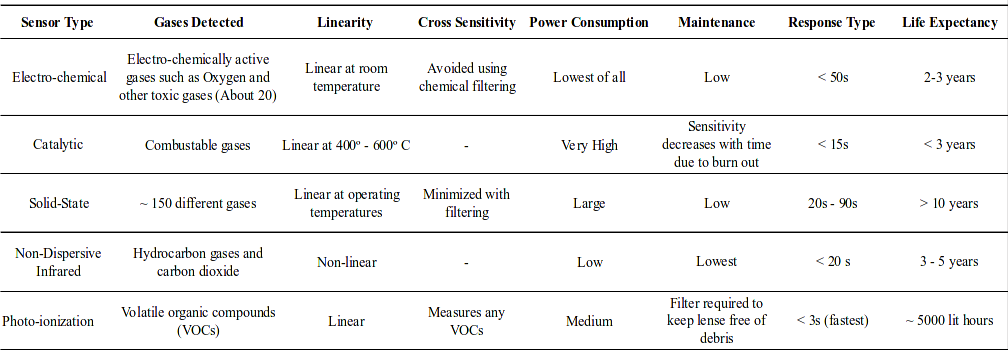
\includegraphics[width=6in]{figures/gas-sensor-comparison.png}
    \caption{A comparison of the different features of gas sensors.}
    \label{gas-sensor-comparison}
\end{figure}


% \begin{table}[H]
% \centering
% \footnotesize	
% \begin{tabularx}{\linewidth}{|X X X X X|}
% \hline
% Sensor Type & Gases Detected & Linearity & Cross Sensitivity & Power Consumption  \\\hline\hline
% Electro-chemical & Electro-chemically active gases such as oxygen and other toxic gasses (about 20) & Linear at room temperature & Avoided using chemical filtering & Lowest of all \\
% Catalytic & Combustable gases & Linear at $400\deg - 600\deg$ C & - & Very high \\ 
% \end{tabularx}
% \vspace{1 cm}
% \begin{tabular}{c c c}
% \hline
% Maintenance & Response Type & Life Expectancy \\\hline\hline
% \end{tabular}



% \label{Gases}
% \caption{Gases}
% \end{table}
\subsubsection{Particulate Matter Sensor}
Particulate matters are small particles dispensed in the air defined by its diameter, usually 10 micrometers or 2.5 micrometers (PM10 and PM2.5). The smaller the particle, the easier it is for it to pierce through the human respiratory and cardiovascular system, making it one of the most dangerous toxins to humans. There are several different ways of detecting particulate matter in the atmosphere. All PM sensors can be categorized under two methods. The first being direct measurement providing continuous readings at predetermined intervals and the other is a laboratory technique using gravimetric analysis. In the laboratory method, a sensor is equipped with a filter that collect ambient particles in the air and is then weighed in a lab and the concentration is calculated. This method is much more time consuming and not feasible for real-time air monitoring systems. The most common methods used in PM detection for air quality measurements are discussed below.

\paragraph{Optical Analysis}
 One method of detecting particulate matter is optical analysis. PM sensors use the principle of laser scattering to track the particles present in the air. A light beam is projected towards a chamber while a fan brings in ambient air into the same chamber. The particles present in the air deflect and scatter the projected light beam and a photodiode then measures how much light passes through the chamber and how much is scattered. A microprocessor embedded within the sensor then converts this measurement into ambient particle concentration. The benefit of these type sensors are that they’re lightweight, battery-operated and small. Optical analysis particulate matter sensors can be further broken down into 3 optical principles:
  
\begin{itemize} 
\item Light Obscuring:
The basic operating principle behind this kind of optical analysis for particulate matter is infrared detection. An infrared emitter such as an LED or light bulb emits light on one side of the chamber while on the other end of the chamber there is an infrared detector. When particulate matter passes through the chamber it obscures some of the light emitted, based on the brightness detected by the sensor, the amount of particles in the air can be detected. Although this method of detection is fast and affordable, it is the least accurate of all the existing methods and cannot distinguish particle diameter (i.e. 2.5 or 10). Air quality can be detected in a binary nature with good or poor, however an exact concentration cannot be given. 
\item Direct Imaging:
A much less common form of detecting particulate matter is through direct imaging with the use of a high-resolution magnifying camera. As particles pass through the chamber the camera records the ambient particles and a computer software analyzes the images for size and count. This is not a method often used in indoor and outdoor pollution monitoring systems as power consumption is much greater when compared to other methods.
\item Light Scatting:
In this kind of optical analysis, a laser beam is used as the primary light source. When the fan brings ambient particles into the chamber that come into contact with the laser beam, the light is scattered, and a photodetector is able to detect the light scatting. The particle count is proportional to the intensity of the scatting light. This is then converted into particle concentration. Laser diffraction for detecting particulate matter is perhaps the best option for this design. In addition to low power consumption, it provides fast and accurate readings as long as the sensor is properly calibrated to distinguish between the diffraction of different particles. 
\end{itemize}

\paragraph{Beta Attenuation Analysis}
 Another way of detecting particulate matter in the air is through beta attenuation mass monitoring. A sample of the ambient air is heated and dried to extract any moisture in the air and then ran through the system and collected by a filter. The filter is then exposed to rays of beta radiation which particulate matters then absorb. The attenuation of the beta rays is then measured determine particle concentration. If properly calibrated and external factors are controlled beta attenuation is an extremely accurate method of detecting particle mass and concentration. However, these machines are large and expensive and only used in laboratory settings and buildings such as the U.S embassy in Beijing. 

\subsubsection{VOC and VSC Sensor}
Volatile Organic Compounds (VOC) and Volatile Sulfur Compounds (VSC) are discharged human-made air pollutants. As defined by the EPA, VOCs are characterized by their high vapor pressure and low water solubility. These emitted gases are often the result of human made chemicals such as paint, benzene, ethylene glycol, petroleum fuels and other factory produced chemicals and aerosols. Studies have shown concentrations of VOCs and VSCs are typically up to 5 times higher in indoor environments than outdoor environments. VOCs and VSCs have a significant role in the contribution to ozone and particulates in the atmosphere and are considered dangerous pollutants to humans. There are several different types of sensors in use today that can measure VOC and VSC concentrations and they vary depending on the type of gas being measured and the industry in which they are used. Some of the common methods used in detecting these type of air pollutants are discussed below.

\paragraph{Photoionization Detector (PID)}
The basic operating principle behind this type of sensor is the use of ultraviolet light to decompose volatile organic compounds into charged ions. Once the particles are broken down a detector then measure the charge of the sampled ionized gas in order to determine concentration. With an average response time of under 3 seconds, this form of detecting VOCs and VSCs is among the fastest. However, power consumption for these devices falls somewhere in the middle when compared to other methods and filtering is required to keep the system free of debris. 

\paragraph{Non-dispersive Infrared Sensing (NDIR)}
With these type of sensors, infrared radiation emitted causes resonance of the sampled gas molecules. Similar to the principle of light scatting, these sensors are equipped with an emitter, a detector, an optical filter, and an electronic module for signal processing. The infrared light passes through a chamber and to a detector, gas particles absorb some of the light and the difference from light emitted to light detected is converted into a gas concentration. NDIR sensors have a higher life-expectancy than electrochemical sensors and are used to detect hydrocarbon pollutants as well as carbon dioxide. 

\paragraph{Flame Ionization Detector (FID)}
This method is widely used in the automotive industry for detecting hydrocarbon emissions as required by government and industry standards. The basic operating principle behind FIDs is ion detection formed from the combustion of organic compounds in a hydrogen flame. A positive and negative electrode are set in place and generate a potential difference, positively charged ions are attracted to the negative plate and when they come in contact with it they produce an electrical current. This current is proportional  to the rate of ionization which can then be related to the concentration of the hydrocarbon. FID sensors are large in size with high power consumption. Because of their operating nature, they also cannot be integrated with other type of gas sensor, hence making it non-ideal for use in the Aether sensing network.

\subsubsection{Sensors Used In Aether}
After sufficient research was done on the different type of sensors that can be used to monitor air quality, the most suitable sensors for the Aether sensing network were selected. These sensors were chosen based on specific characteristics including:

\begin{itemize}
\item Size
\item Power Consumption
\item Integratebility
\item Cost
\item Gas Sensitivity
\end{itemize}

There will be 3 main sensors used in this design, a particulate matter (PM2.5) sensor, an ozone/nitrogen dioxide sensor, and a multi-gas VOC/VSC sensor capable of detecting several gases through machine learning (ML) algorithms as well as measuring ambient temperature and humidity. These sensors are discussed in further detail below
\paragraph{Sensirion SPS30 – Particulate Matter Sensor}
The Sensirion SPS30 sensor is a particulate matter sensor designed for use in air quality monitoring system applications. It’s an optical PM sensor using the principle of laser scattering to detect particulate matter concentrations of varying diameters including PM1.0, PM2.5, PM4 and PM10. With an expected lifetime of over 8 years, the SPS30 sensor provides reliable consistent use without the need for cleaning or maintenance, making it an ideal choice for a stationary indoor/outdoor air quality monitoring system such as Aether.

The SPS30 operates off a laser-based scattering principle alongside sophisticated algorithms to provide accurate measurements for different kinds of particulate matters in the atmosphere. It has a mass concentration range of 0 to 1,000 $\mu$g/$m^3$ with a +/- 10\%  accuracy. EPA standards list acceptable 24-hr average PM concentrations can reach up to 35 $\mu$g/m3 making the sensor range more than capable of detecting dangerous levels of particulate matter. As previously stated, the SPS30 can detect particulate matters of varying diameters including PM1.0, PM2.5, PM4 and PM10. It’s lowest limit of detection for PM is 0.3 micrometers with a minimum sampling interval of 1s when on continuous mode and an operating temperature ranging from -10 to 60º C. The sensor dimensions of 40.6 x 40.6 x 12.2 mm3 provide a small ultra-compact package that allow for easy integration onto the Aether sensing network, contributing to a smaller more compact overall design. It’s compatible with both UART and \iic interfaces and requires a constant voltage supply of 4.5-5.5 V. The design outline and table of specification obtained from Sensirion’s SPS30 datasheet can be seen below.
	
	%need to insert figures%
\paragraph{Renesas ZMOD4510 – \ndo/\ozone Gas Sensor }
The Renesas ZMOD4510 is a solid-state gas sensor that utilizes a heating element on a MEMS structure and a MOx resistor to detect gases. An IC regulates the temperature of the heating element and measures the resistance across the MOx resistor which is a function of the accumulation of ions resulting in the interaction of targeted gas molecules and the metal oxides. This change in conductivity measured is then converted to gas concentration in the ambient air. The device can be used in several different indoor and outdoor applications but is ideal for measuring outdoor air quality. It’s equipped with 2 different sensor outputs based on the selected operating method, a non-selective ozone and nitrogen dioxide reading or a selective ozone-only reading using the chips ultra-low power mode.

The ZMOD4510 is a 12-pin LGA assembly with dimensions of 3.0 × 3.0 × 0.7 mm. It uses an I2C communication link supporting up to 400kHz with an average low power consumption of 0.2 mW making it an ideal choice for use in this design. The sensor’s operating temperature ranges from -40°C to +65°C and requires a supply voltage of 1.7V – 3.6V. In its first operation mode, although not able to detect gas concentrations of other gases the ZMOD4510 sensor module is capable of directly calculating the AQI based on EPA standards. It does this by using embedded artificial intelligence (AI) and machine learning (ML) algorithms to detect several gases in the atmosphere. Additionally, its second mode of operation is a selective O3 measurement using a low power mode. This provides flexibility to the overall design of the system, as it can be used to directly calculate AQI or just have the sensor output an Ozone concentration reading and using that along with the other sensors in Aether to calculate the AQI. The different measurement capabilities and characteristics of the ZMOD4510 sensor  based on its selected operation method are shown in the figure below. 

%need to insert figures%
\paragraph{Bosch BME688 Gas Sensor – VOCs and VSCs}
The Bosch BME688 detects Volatile Organic Compounds (VOCs) and Volatile Sulfur Compounds (VSCs) and through the use of sophisticated AI embedded in the system, machine learning algorithms can be implemented to detect a variety of other gases and compounds including carbon monoxide (CO2) and hydrogen. Additionally, through the use the BME AI studio provided by Bosch, the sensor can be customized and trained to detect different smells such as methane or smoke making the overall design of the Aether much more flexible and capable of detecting early on set symptoms of methane leaks, fires, and other smells hazardous to humans. BME688 also provides consistent and stable temperature and humidity readings eliminating the need to integrate another sensor onto the design and thus saving time and space. Since VOC and VSC concentrations are always higher in indoor environments, it gives the Aether sensing network the ability to be an effective indoor air quality IoT sensing system while also contributing to its ability to measure the AQI in outdoor environments. 

The BME688 is enclosed in an 8-pin LGA assembly with dimensions of 3.0 x 3.0 x 0.93 mm3 making it an extremely compact design. This allows Aether to add several robust sensing features while keeping the overall design as compact and portable as possible. It uses an \iic or SPI communication link with an operating supply voltage of 1.2 V – 3.6 V. Its temperature detecting ranges from -40°C to +85°C and can detect ambient humidity up to 100\% . The gas sensors and humidity sensor response times are both under 11 s contributing to fast and accurate measurements. To achieve the sensors full operating potential, the Bosch Sensor Environmental Cluster (BSEC) and BME6xy API will need to be used to train the sensor to detect the required gases and smells. BME688 is equipped with 5 different operating modes.

\begin {itemize}
\item Gas Scan Mode: Using the BME AI Studio the sensor can be trained to scan and detect selective gases for AQI and indoor air quality applications with a 10.8s refresh scan rate.
\item Ultra-Low Power (ULP):  This mode is designed for use for battery-powered operation over longer periods of time. It operates the sensor with a <1.0mA consumption and a 300s refresh rate.
\item Quick Ultra-Low Power (q-ULP): This mode detects temperature, pressure and humidity with a 3s refresh rate and a not much higher current consumption.
\item Low-Power (LP): Designed specifically for an interactive application tracking air quality, this mode has a 3s refresh rate with a <1.0 mA current consumption. 
\item Continuous (CONT): With an update rate of 1 Hz, this mode is intended for use in short-term uses where extremely fast events occur and fast responses are needed. 

\end {itemize}
The overall design of this product allows it to be used in battery-powered IoT applications where size and power consumption are of paramount importance. At a price of \$20 its low cost allows the design to have much more capability and flexibility in its measurements while keeping the total product cost relatively low.

\subsubsection{Other Sensors Considered}
This section discusses different sensors that were considered for this project but ultimately not used. Initially, the thought process behind having an air pollution detection network was to use an individual gas sensor for each different gas detected in order to calculate the AQI Index. As more research was done, it became obvious that using a separate gas sensor for each pollutant would unnecessarily complicate integration onto the system while increasing power consumption, cost, and overall product dimensions. Some of the sensors considered for the Aether sensing network are discussed below.
\paragraph{\textit Spec Sensors - Multigas}
\paragraph{}
The company Spec Sensors produces a variety of high performance, ultra-low power consumption electrochemical gas sensors. As discussed in the sections above, electrochemical based gas sensors typically have a lifespan of approximately 1-3 years, significantly less than other sensors researched, making the overall design unideal for long-term low maintenance use. Additionally, these sensors are also cross-sensitive to other gases and because a variety of different gases will be measured in this design, the likelihood of inaccurate readings would be increased. Electrochemical sensors base their measurements off  electrochemical reactions which are temperature dependent. Although the built-in sensor design compensates for temperature changes, rapid changes in temperature and humidity may cause all the sensors in the system to temporarily destabilize and affect product performance. At a cost of 20 (USD) per gas sensor, using Spec Sensors for monitoring air quality in our design would have also increased overall product cost while not providing much flexibility in design capabilities and making circuit integration more difficult. 

\paragraph{\textit Sensirion AG – Temperature and Humidity}

\paragraph{}
Initially for this design, a separate sensor intended for specifically monitoring ambient temperature and humidity was going to be used. However, after conducting more research on available products, the Bosch BME688 would not only provide readings for VOCs and VSCs but could also provide stable and consistent temperature and humidity measurements. Thus, eliminating the need to integrate another sensor onto the PCB design thus further limiting the cost and size of the overall product. 
\paragraph{}
After considering different sensors and the different operating principles they used to detect gases, it was determined the best course of action would be to use sensors that have low power consumptions while also having the ability to detect more than one type of gas. This would allow for the system to use less sensors and minimize the size of the main PCB. The Bosch BME688 uses built in machine learning software and is capable of being trained to detect VOC/VSCs, temperature and humidity, and a variety of different gases. Although not able to provide direct measurements for other gases, it still gives the system the ability to detect harmful air pollutants. The Renesas ZMOD4510 sensor used in the design can measure both Nitrogen Dioxide and Ozone which re to of the most prevalent air pollutants used in calculating the AQI Index. 
